\documentclass[12pt,letterpaper]{article}
\usepackage[moduleName={Fourier},version={2.1.2}]{ArhythmeticUnits}

\input{PanelDrawing.tex}

\begin{document}
\titlePage{img/Logo}{img/PanelLayout.png}{img/ArhythmeticUnits}{}
\section*{Using This Manual}
Start with Quick Start to get a signal on screen. The numbered panel drawing
is a map to the control reference. The walkthroughs then turn those controls
into experiments: patch a source, choose a known setup, change one thing,
and interpret the result.

\begin{center}
\renewcommand{\arraystretch}{1.3}
\begin{tabularx}{\textwidth}{@{}Xr@{}}
\toprule
\textbf{Find your way} & \textbf{Page} \\
\midrule
\hyperref[sec:overview]{Overview} & \pageref{sec:overview} \\
\hyperref[sec:quick-start]{Quick Start} & \pageref{sec:quick-start} \\
\hyperref[sec:panel]{Panel Layout And Controls} & \pageref{sec:panel} \\
\hyperref[sec:display]{Reading The Display} & \pageref{sec:display} \\
\hyperref[sec:settings]{Context Menu And Saved Settings} & \pageref{sec:settings} \\
\hyperref[sec:harmonics]{Hearing Harmonics} & \pageref{sec:harmonics} \\
\hyperref[sec:filter]{Comparing A Filter} & \pageref{sec:filter} \\
\hyperref[sec:resolution]{Separating Nearby Tones} & \pageref{sec:resolution} \\
\hyperref[sec:measurements]{Making Useful Measurements} & \pageref{sec:measurements} \\
\hyperref[sec:presets]{Factory Presets} & \pageref{sec:presets} \\
\hyperref[sec:control-values]{Control Values (Reference)} & \pageref{sec:control-values} \\
\hyperref[sec:troubleshooting]{Troubleshooting} & \pageref{sec:troubleshooting} \\
\hyperref[sec:further-reading]{Analysis Timing And Further Reading} & \pageref{sec:further-reading} \\
\bottomrule
\end{tabularx}
\end{center}

\paragraph{Try the experiments}
Use any Rack modules that provide the named functions; no particular
oscillator, filter, or envelope is required. Settings in the walkthroughs
are starting points, not new factory presets. Values in milliseconds and
hertz assume the stated Rack sample rate. Keep your listening path connected
separately: the analyzer has no audio outputs.

\paragraph{Keep comparisons fair}
Use the same source and sample rate, match input gains, and set Slope to zero
before comparing levels. Change one control at a time. Schematic figures
explain relationships rather than reproduce captured data; the cover shows
the rendered module.

\clearpage

% ----------------------------------------------------------------------------
% MARK: Overview
% ----------------------------------------------------------------------------

\section{Overview}\label{sec:overview}

\textbf{Fourier} is a four-input spectrum analyzer for VCV Rack 2. It shows
how a signal's amplitude is distributed across frequencies. Each input has
its own gain control and colored trace; the analysis and display controls
are shared by all four inputs. Fourier has no audio outputs: patch a signal
to it alongside your audio path to inspect the signal without changing it.

The analyzer uses a short-time Fourier transform (STFT), with selectable
window functions, FFT lengths, and intervals between analyses. Time and
frequency smoothing help reveal broad trends, while frequency bounds and
amplitude scales let you inspect a smaller part of the spectrum. A slope
control tilts the displayed amplitudes around $1\,\mathrm{kHz}$.

Fourier and Spectre belong to the Arhythmetic Units Fourier plugin.
Use Fourier to compare the current spectra of up to four signals, and
Spectre to follow one signal's spectrum over time. Both provide the same
window choices and smoothing controls, but their display axes, input-gain
defaults, and Run behavior differ as described below.

The module takes its name from Jean-Baptiste Joseph Fourier
(Fig.~\ref{fig:fourier-portrait}), whose work describes signals in terms of
simpler trigonometric functions.

\begin{figure}[!htp]
\centering

\includegraphics[width=0.38\textwidth]{img/FourierPortrait}
\caption{Jean-Baptiste Joseph Fourier (March 1768 -- May 1830).}
\label{fig:fourier-portrait}
\end{figure}

\clearpage
\section{Quick Start}\label{sec:quick-start}

\begin{itemize}
  \item Connect an oscillator or other audio source to the red input. Keep
  your existing connection to the mixer or audio output if you want to hear it.
  \item Leave the input gain at $0\,\mathrm{dB}$ and ensure \textbf{Run} is lit.
  A new module uses a Flattop window, Length 2048, and Hop
  $30\,\mathrm{ms}$, with no time or frequency smoothing.
  \item For an amplitude comparison, set \textbf{Slope} to
  $0\,\mathrm{dB/oct}$. The default $+4.5\,\mathrm{dB/oct}$ visually boosts
  frequencies above $1\,\mathrm{kHz}$ and reduces those below it.
  \item Connect another signal to the green, blue, or yellow input to
  compare spectra. Use equal input gains for a level comparison.
  \item Hover over the plot to show a crosshair, frequency, musical note
  and tuning offset, and amplitude at the cursor position. The readout
  describes the cursor; it does not automatically find a spectral peak.
  \item Press \textbf{Run} to stop capturing new samples. Press it again
  to resume. The retained audio can still be reanalyzed while capture is stopped.
\end{itemize}

\paragraph{Reading levels}
Fourier displays spectral magnitudes, not total signal RMS, loudness, or
sound pressure level. Its nominal amplitude reference is a
$5\,\mathrm{V}$ peak sine wave (approximately $0\,\mathrm{dB}$ or
$100\,\%$ with unity gain, zero slope, and no smoothing). Window choice,
frequency alignment with FFT bins, and smoothing affect the height and width
of a peak. The display ceiling is about $+12\,\mathrm{dB}$; a trace reaching
that ceiling does not mean Fourier has clipped your audio path.

\paragraph{Choosing settings}
Use a longer \textbf{Length} to separate nearby frequencies, especially in
the bass. Use a shorter \textbf{Hop} and little or no \textbf{Average} to
follow changes more closely. Increase \textbf{Average} for a steadier trace
and \textbf{Smooth} for a broader view of tonal balance. The factory presets
provide examples of these choices.

% ----------------------------------------------------------------------------
% MARK: Panel Layout
% ----------------------------------------------------------------------------

\clearpage
\section{Panel Layout}\label{sec:panel}

\begin{figure}[!htp]
\centering
\resizebox{\textwidth}{!}{% Conceptual control groups, not a second rendering of the module UI.
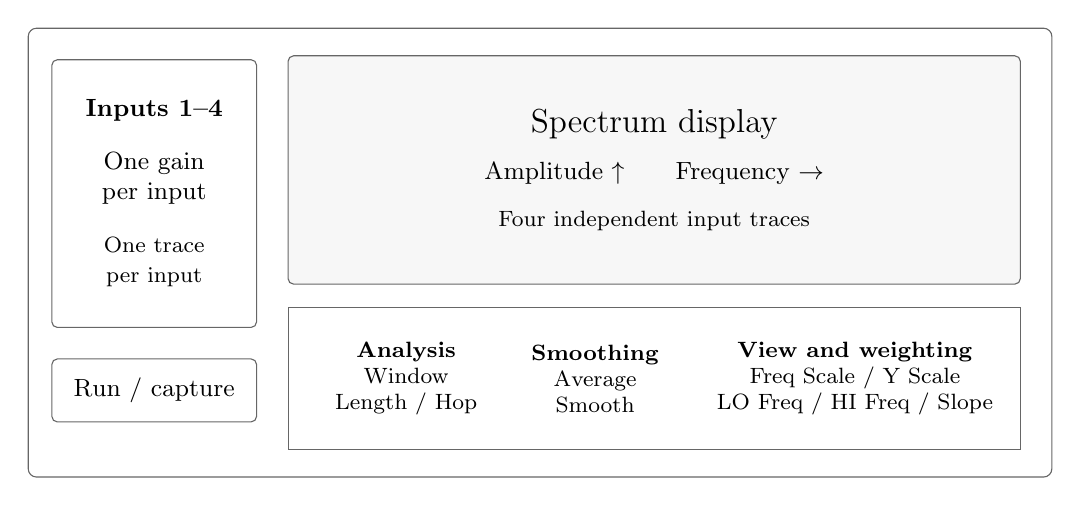
\begin{tikzpicture}[x=1cm,y=1cm,font=\small,
    region/.style={draw=black!60,rounded corners=2pt,align=center},
    label/.style={font=\footnotesize,align=center}]
  \draw[black!60,rounded corners=3pt] (0,0) rectangle (13,5.7);
  \node[region,minimum width=2.6cm,minimum height=3.4cm] at (1.6,3.6)
    {\textbf{Inputs 1--4}\\[8pt]One gain\\per input\\[8pt]
      \footnotesize One trace\\\footnotesize per input};
  \node[region,minimum width=2.6cm,minimum height=.8cm] at (1.6,1.1)
    {Run / capture};
  \node[region,fill=black!3,minimum width=9.3cm,minimum height=2.9cm]
    at (7.95,3.9) {\large Spectrum display\\[6pt]
      Amplitude $\uparrow$\qquad Frequency $\rightarrow$\\[6pt]
      \footnotesize Four independent input traces};
  \draw[black!60] (3.3,.35) rectangle (12.6,2.15);
  \node[label] at (4.8,1.25) {\textbf{Analysis}\\Window\\Length / Hop};
  \node[label] at (7.2,1.25) {\textbf{Smoothing}\\Average\\Smooth};
  \node[label] at (10.5,1.25) {\textbf{View and weighting}\\Freq Scale / Y Scale\\LO Freq / HI Freq / Slope};
\end{tikzpicture}
}
\caption{Panel reference. Numbered callouts match the control sections
below. The screen and value fields are schematic; the cover shows the module
in operation.}
\end{figure}

Each input and gain pair controls one trace. The lower strip controls the
analysis and display for all four inputs. The reference shows control
locations without prescribing settings. Text controls brighten when hovered.

\begingroup
\setlength{\parindent}{0pt}
\setlength{\parskip}{4pt}
\colorlet{panelAccent}{fourierAccent}
\clearpage
\subsection{Input}

Patch a signal to an input to see its spectrum. The four inputs run from
red at the top through green, blue, and yellow. Each has its own trace and
gain knob, so you can compare up to four signals with the same analysis
settings. Leave the gains at \textbf{0 dB} for a fair level comparison.

Gain changes what Fourier analyzes; it does not change what you hear through
your existing audio path. Turning it fully down silences that input's
analysis. The maximum, +12 dB, is about four times the input amplitude.

A polyphonic cable is combined into one signal at each jack. Voices are not
shown separately: they can reinforce or cancel one another. Split voices
into separate cables if you want to compare them individually.

\subsection{Run}

\textbf{Lit: capture new audio. Dark: inspect the audio already captured.}
Press Run to stop following a changing sound, then experiment with the
analysis settings. Press it again to resume. Run starts enabled.

Stopping capture does not stop Fourier's analysis. The last unfinished
analysis may complete, and Average can continue to settle. This makes Run
useful for comparing windows on the same retained sound.

\begin{center}
\renewcommand{\arraystretch}{1.35}
\begin{tabularx}{\textwidth}{@{}p{.35\textwidth}X@{}}
\toprule
\textbf{While Run is off} & \textbf{What happens} \\
\midrule
Window, Average, Smooth & Reanalyze the retained audio. \\
Scales, bounds, Slope & Change how the result is displayed. \\
Gain, AC coupling & Resume capture to see their effect in the analysis. \\
Length & Clears the retained audio; resume to fill it again. \\
\bottomrule
\end{tabularx}
\end{center}

\paragraph{Try it}
Capture a steady oscillator, stop Run, and switch Window between Hann and
Flattop. Watch the width of the peak change even though the captured sound
has not changed. The next page explains why.

\clearpage
\subsection{Window Function}
A pure tone does not always appear as one thin line. The analyzer works on
short pieces of audio, and the edges of each piece can spread the tone into
nearby frequencies. This spreading is called \textit{leakage}. A window
softens the edges, trading a broader main peak for less energy around it.

\textbf{Start with Flattop} when comparing the heights of steady tones.
Try \textbf{Hann} when you want to distinguish nearby harmonics. Boxcar gives
a narrow main peak, but its leakage can hide quieter tones beside a loud one.
No window is best for every sound. The FFT measures at evenly spaced
frequencies called \textit{bins}; the plots below show what it sees.

\begin{figure}[!htp]
\centering
\input{WindowTradeoffs.tex}
\caption{Calculated responses to one tone halfway between FFT bins.
The dashed line marks the tone; dots mark measured bins. All three plots use
the same 2048-sample length and level scale. The ripples are leakage, not
additional tones.}
\end{figure}

\paragraph{Read the shape, not just the height}
The small ripples around a large peak can come from the analysis itself;
they are not necessarily extra notes or noise in the source. Compare windows
before drawing that conclusion. The module compensates for the window's
level reduction, but peak shape and the displayed noise level still change.

\paragraph{Try it}
With Average and Smooth off, move an oscillator's pitch slowly. Flattop
usually gives a steadier peak height as the tone passes between bins;
Hann gives a narrower peak. Fourier can also compare these windows while
Run is off. The complete window menu is on page~\pageref{sec:control-values}.

\clearpage
\subsection{Length}

\textbf{Length decides how much audio goes into one spectrum.} A longer
piece helps separate nearby pitches, especially in the bass. A shorter piece
follows a changing sound more closely. Start at the default \textbf{2048}
samples, then increase Length when two nearby tones merge into one peak.

\begin{figure}[!htp]
\centering
% Derived geometry at 48 kHz: frame duration N/fs and bin spacing fs/N.
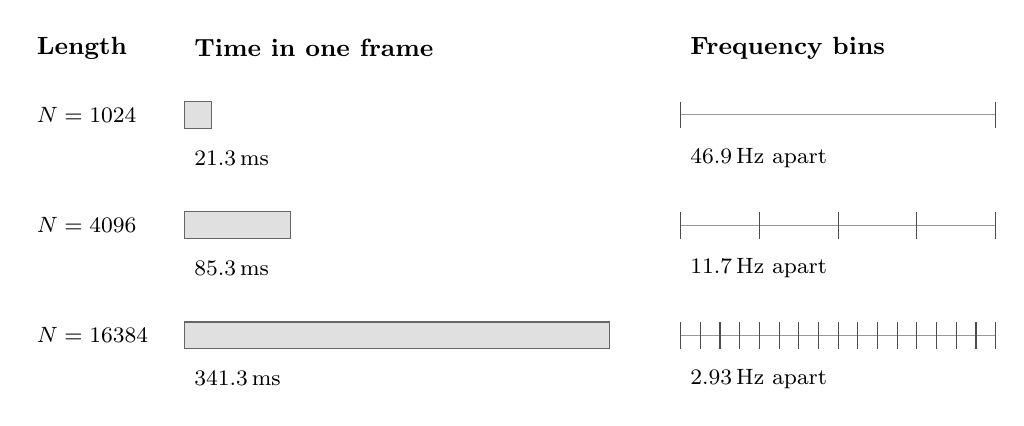
\begin{tikzpicture}[x=1cm,y=1cm,font=\footnotesize]
  \node[anchor=west,font=\small\bfseries] at (0,3.65) {Length};
  \node[anchor=west,font=\small\bfseries] at (2,3.65) {Time in one frame};
  \node[anchor=west,font=\small\bfseries] at (8.3,3.65) {Frequency bins};
  \foreach \n/\intervals/\y in {1024/1/2.8,4096/4/1.4,16384/16/0} {
    \node[anchor=west] at (0,\y) {$N=\n$};
    \pgfmathsetmacro{\duration}{5.4*\intervals/16}
    \draw[fill=black!12,draw=black!60] (2,\y-.17) rectangle +(\duration,.34);
    \draw[black!40] (8.3,\y) -- (12.3,\y);
    \foreach \k in {0,...,\intervals} {
      \pgfmathsetmacro{\x}{8.3+4*\k/\intervals}
      \draw[black!70] (\x,\y-.17) -- (\x,\y+.17);
    }
  }
  \node[anchor=west] at (2,2.25) {$21.3\,\mathrm{ms}$};
  \node[anchor=west] at (2,.85) {$85.3\,\mathrm{ms}$};
  \node[anchor=west] at (2,-.55) {$341.3\,\mathrm{ms}$};
  \node[anchor=west] at (8.3,2.25) {$46.9\,\mathrm{Hz}$ apart};
  \node[anchor=west] at (8.3,.85) {$11.7\,\mathrm{Hz}$ apart};
  \node[anchor=west] at (8.3,-.55) {$2.93\,\mathrm{Hz}$ apart};
\end{tikzpicture}

\caption{The tradeoff at a Rack sample rate of 48 kHz. A longer frame includes
more time and gives more closely spaced frequency bins. Each row shows the
same time and frequency spans. Window choice also affects whether two tones
can be separated.}
\end{figure}

A \textit{bin} is one of the evenly spaced frequencies measured by the FFT.
More bins can reveal finer detail; enlarging the view alone cannot. Longer
frames also require more computation. Changing Length clears the captured
audio, so leave Run on long enough to collect a new frame.

\subsection{Hop}

\textbf{Hop decides how often to start another spectrum.} Its default is
\textbf{30 ms}. Lower values follow changes with more frequent analyses;
higher values reduce the analysis workload. The available range is 5--300 ms.

Length and Hop do different jobs. Imagine taking overlapping photographs:
Length is the time covered by each exposure, and Hop is the time between
exposures. Reducing Hop does not shorten the audio inside each frame.
If Hop is longer than a frame, gaps appear between the analyzed pieces and
a short event can be missed. Rack's display refresh also affects when you
see an update; Hop is not a promise of screen latency.

\clearpage
\subsection{Freq Scale}

Choose \textbf{Linear} to compare harmonic spacing: equal steps in hertz
occupy equal widths. \textbf{Logarithmic} (the default) gives the bass more
room. This version uses a square-root mapping, so octaves are not equally
wide; read the labels or hover readout for exact frequencies.

\subsection{Y Scale}

Start with \textbf{Log 60dB} for everyday use. Choose \textbf{Log 120dB}
to see quieter detail. Both extend up to +12 dB; their names identify the
lower limit. \textbf{Linear} emphasizes large amplitudes, expressed as
percentages. Changing scale changes the view, not the sound.

\subsection{Average}

Increase \textbf{Average} to calm a flickering trace and compare broad trends.
Leave it at \textbf{0 ms} to follow attacks. Higher settings give previous
results more influence; they do not select a fixed-length recording. The
range extends to 2500 ms.

\subsection{Smooth}

Leave \textbf{Smooth} at \textbf{None} for individual harmonics. Try
\textbf{1/12 octave} for a gentler outline of tonal balance. Wider settings
merge neighboring peaks and can lower them; they do not add resolution.
The octave-based width covers more hertz in the treble than in the bass.

\begin{figure}[!htp]
\centering
\input{Smoothing.tex}
\caption{Average softens changes across time; Smooth blends detail across
frequency. These are qualitative sketches, not measured responses.}
\end{figure}

\clearpage
\subsection{Low Frequency}

\textbf{LO Freq} sets the left edge of the plot. Raise it to leave frequencies
below your area of interest out of the view. It starts at \textbf{0 Hz}.
This is a viewing control, not a high-pass filter on the sound.

\subsection{High Frequency}

\textbf{HI Freq} sets the right edge. Lower it to give the bass or a group of
harmonics more room. Keep it above LO Freq. Both controls can reach half of
Rack's sample rate, called the \textit{Nyquist frequency}; that is 24 kHz
at a 48 kHz sample rate. HI Freq starts at this upper limit.

\paragraph{Try it}
Set LO Freq to 0 Hz and HI Freq to 500 Hz to inspect the bass. The existing
peaks spread across a wider area, but no new frequency detail is added.
If nearby tones still merge, increase Length. Check your bounds after
changing Rack's sample rate, because the available range changes too.

\subsection{Slope}

\textbf{Slope tilts the view, like a display-only tone control.} Positive
values lift high frequencies and reduce low frequencies around a 1 kHz
pivot. Negative values reverse that tilt. Your audio is unaffected.

The default is \textbf{+4.5 dB per octave}, which can help show high-frequency
content. Set it to \textbf{0} when comparing unweighted levels. Its range is
$-9$ to $+9$ dB per octave.

\begin{center}
\renewcommand{\arraystretch}{1.3}
\begin{tabular}{@{}lrrr@{}}
\toprule
\textbf{Example: +3 dB/oct} & \textbf{500 Hz} & \textbf{1 kHz} & \textbf{2 kHz} \\
\midrule
Change in displayed level & $-3$ dB & 0 dB & $+3$ dB \\
\bottomrule
\end{tabular}
\end{center}

An octave doubles the frequency. The same tilt continues above and below
the example: it is not an equalizer acting on the source. Input gain,
windowing, and smoothing can also change the displayed levels; keep those
settings fixed when judging what Slope does.

\endgroup


\clearpage
\section{Reading The Display}\label{sec:display}

Frequency runs from left to right and spectral amplitude from bottom to top.
Each colored trace represents one input port's summed signal. Input gain,
windowing, smoothing, and Slope affect the trace; use equal gains and zero
slope for unweighted comparisons.

The crosshair and readouts appear only inside the plot rectangle. Moving
onto the surrounding labels or control strip hides them.

Hover over the plot for a crosshair and readouts of frequency, musical note,
tuning offset, and amplitude. The amplitude describes the cursor's vertical
position on the selected Y Scale; place it on a trace to read that trace's
level. It does not automatically find a peak. Spectre's hover readout instead
measures a stored spectral bin at the selected time and frequency, before
Slope weighting.

\section{Context Menu And Saved Settings}\label{sec:settings}

Right-click the module to find these options under \textbf{Render Settings}:
\begin{itemize}
  \item \textbf{Filled Display} shades the area beneath each trace. It is
  off by default.
  \item \textbf{Bezier Curve} draws curved connections between the plotted
  points. It is on by default. Turning it off uses straight segments and can
  make individual bins easier to inspect. It does not change FFT resolution.
  \item \textbf{AC-coupled} removes DC offset from newly captured inputs
  using a DC-blocking filter. It is on by default and can also affect very
  low frequencies. Turn it off when inspecting DC or slow signals, and set
  Slope to zero to avoid frequency weighting near DC.
\end{itemize}

These three menu changes support Rack's Undo and Redo commands. Panel
settings, menu options, and the running state are saved with patches and
presets. The captured audio and spectrum are not saved. Loading a patch
that was saved with Run off therefore does not restore a frozen trace;
press Run to capture a new one.

Rack's module initialization resets the controls to their defaults, enables
Run, AC coupling, and Bezier curves, and disables Filled Display.

\clearpage
\section{Hearing Harmonics}\label{sec:harmonics}

A spectrum connects a sound's timbre to its partials. Try this with an
oscillator that offers sine, triangle, saw, and square outputs at one pitch.

\paragraph{Starting point}
Load \textbf{Harmonics}. Set all input gains to $0\,\mathrm{dB}$, Length
4096, Hop $30\,\mathrm{ms}$, and Y Scale to Log 60dB. Keep Average and
Smooth off, Slope at zero, and the view at $0$--$5\,\mathrm{kHz}$.
Tune the oscillator near $220\,\mathrm{Hz}$; exact tuning is not required.

\begin{enumerate}
  \item Patch sine to red and saw to green. Look for a shared lowest peak,
  the fundamental. The saw should have peaks near integer multiples of it:
  $440$, $660$, $880\,\mathrm{Hz}$, and so on.
  \item Patch triangle to blue and a square with 50\% pulse width to yellow.
  Compare peaks near $3f_0$ and $5f_0$. An ideal triangle's upper harmonics
  fall faster than a square's; both lack even harmonics.
  \item Change the pulse width. Even harmonics can now appear, and some
  harmonics weaken or disappear. Listen while watching the pattern change.
  \item Increase Smooth, then return it to None. The broad tonal shape is
  easier to compare when smoothed, but individual partials merge.
\end{enumerate}

\begin{figure}[!htp]
\centering
% Ideal relative partial amplitudes, independent of module UI and FFT results.
\begin{tikzpicture}[x=1cm,y=1cm,font=\small]
\foreach \origin/\title/\mode in {0/Saw/1,4.5/Square/2,9/Triangle/3} {
  \begin{scope}[shift={(\origin,0)}]
    \node[anchor=west,font=\small\bfseries,text=fourierAccent] at (0,2.25) {\title};
    \draw[->,panelMuted] (0,0)--(3.85,0);
    \draw[->,panelMuted] (0,0)--(0,1.85);
    \foreach \n in {1,...,7} {
      \pgfmathsetmacro{\amp}{\mode==1 ? 1/\n : (mod(\n,2)==0 ? 0 : (\mode==2 ? 1/\n : 1/(\n*\n)))}
      \draw[fourierAccent,line width=1.2pt] (\n*.45,0)--(\n*.45,\amp*1.65);
      \fill[fourierAccent] (\n*.45,\amp*1.65) circle[radius=.035];
    }
    \node[below] at (.45,0) {$f_0$};
    \node[below] at (1.35,0) {$3f_0$};
    \node[below] at (2.25,0) {$5f_0$};
    \node[below] at (3.15,0) {$7f_0$};
  \end{scope}
}
\end{tikzpicture}

\caption{Ideal harmonic amplitudes relative to each waveform's fundamental.
Stems indicate discrete partials, not the broadened peaks of a finite FFT.
Real oscillators may intentionally depart from these shapes.}
\end{figure}

\paragraph{What to learn}
Peak spacing reveals harmonic structure; relative heights help explain
brightness. Equal peak voltage at the oscillator outputs does not guarantee
equal fundamental height or perceived loudness. To compare only spectral
shape, temporarily adjust analyzer input gains to align the fundamentals.
Return to equal gains before making a level comparison. A missing peak may
also lie below the selected Y Scale or be hidden beneath another trace.

\clearpage
\section{Comparing A Filter}\label{sec:filter}

Use two inputs to see what a processor changes while keeping the source
identical. A low-pass filter and a steady saw or noise source are enough.

\begin{figure}[!htp]
\centering
% Functional routing diagram, not a Rack patch screenshot.
\begin{tikzpicture}[x=1cm,y=1cm,font=\small,
  block/.style={draw=panelRule,rounded corners=2pt,fill=panelPaper,
    minimum width=2.3cm,minimum height=.8cm,align=center},
  wire/.style={-{Stealth[length=5pt]},line width=.9pt,draw=panelInk}]
  \node[block] (source) at (1.3,2) {Saw / noise};
  \node[block] (filter) at (6,2) {Filter};
  \node[block] (listen) at (11,2) {Listening path};
  \node[block,draw=channelOne] (red) at (3.6,0) {Fourier: red};
  \node[block,draw=channelTwo] (green) at (8.4,0) {Fourier: green};
  \draw[wire] (source)--(filter);
  \draw[wire] (filter)--(listen);
  \fill[panelInk] (3.6,2) circle[radius=.06];
  \fill[panelInk] (8.4,2) circle[radius=.06];
  \draw[wire,draw=channelOne] (3.6,2)--(red);
  \draw[wire,draw=channelTwo] (8.4,2)--(green);
  \node[above,text=panelMuted] at (3.6,2.1) {Before};
  \node[above,text=panelMuted] at (8.4,2.1) {After};
\end{tikzpicture}

\caption{Tap the signal before and after the filter. Analyzer cables are
branches of the listening path; Fourier is not an audio effect.}
\end{figure}

\paragraph{Starting point}
Load \textbf{Mastering}, then set Slope to zero and Smooth to None. Use
$0\,\mathrm{dB}$ gain on both connected inputs. Keep Length 4096 and
Hop $30\,\mathrm{ms}$. Choose Average $300\,\mathrm{ms}$ for noise, or
turn it off for a steady saw. Start with low filter resonance.

\begin{enumerate}
  \item Branch the source to the red input and the filter input. Patch
  the filter output to green and to your listening path.
  \item With the cutoff high, compare levels well below the cutoff. A
  constant difference here can be the filter's passband gain; it is not
  necessarily a change in spectral shape.
  \item Lower the cutoff slowly. The green trace should fall below red at
  higher frequencies. Raise resonance to look for a peak near the cutoff.
  Wait for Average to settle after each change.
  \item At a frequency with useful energy in both traces, place the cursor
  on each trace and subtract their dB levels. If red is $-12\,\mathrm{dB}$
  and green is $-24\,\mathrm{dB}$, the observed change is $-12\,\mathrm{dB}$:
  about one quarter of the amplitude at that frequency.
\end{enumerate}

\paragraph{Read the comparison carefully}
A saw samples the response only at its harmonics; noise fills more of the
spectrum but fluctuates. The ratio becomes unreliable where the source is
very weak. Fourier does not divide traces or measure phase automatically.
This is a visual magnitude comparison, not a complete transfer-function
measurement. Saturation, modulation, or other nonlinear behavior can create
new harmonics, so the result then depends on the source and its level.

\paragraph{Go further}
Use blue for a second filter or processing stage. Keep analyzer gains equal
and compare all taps simultaneously. Disable Filled Display if overlapping
areas obscure the curves. A processor's latency can make changing sounds
appear at different stages of their envelope; use a steady sound first.

\clearpage
\section{Separating Nearby Tones}\label{sec:resolution}

Two low notes can look like one broad peak. This experiment distinguishes
frequency resolution from simply enlarging the display.

\paragraph{Starting point}
Use two sine oscillators near $100$ and $110\,\mathrm{Hz}$, summed through
a mixer into red. At a Rack sample rate of $48\,\mathrm{kHz}$, choose Hann,
Length 2048, Hop $30\,\mathrm{ms}$, Linear Freq Scale, and
$0$--$300\,\mathrm{Hz}$. Set Average and Smooth off and Slope to zero.

\begin{enumerate}
  \item Observe the mixture, then mute each oscillator in turn to locate
  its contribution. At Length 2048 the two tones are closer than one bin.
  They will be difficult to distinguish in the mixture.
  \item Restore both tones and increase Length to 16384. Allow fresh audio
  to fill the new frame. The finer bin spacing should make them easier to
  separate with Hann; a broader window such as Flattop may still merge them.
  \item Return to Length 2048 and narrow LO/HI Freq around the peaks.
  The existing shape grows on screen, but the missing detail does not return.
  Turn off Bezier Curve in the context menu to see the bin connections.
  \item Return to Length 16384 and change one oscillator's pitch abruptly.
  Notice the transition taking time to pass through the long frame. A smaller
  Hop updates more frequently but does not shorten that frame.
\end{enumerate}

\begin{center}
\renewcommand{\arraystretch}{1.25}
\begin{tabular}{@{}rrr@{}}
\toprule
\textbf{Length at 48 kHz} & \textbf{Audio span} & \textbf{Bin spacing} \\
\midrule
2048 & $42.67\,\mathrm{ms}$ & $23.44\,\mathrm{Hz}$ \\
4096 & $85.33\,\mathrm{ms}$ & $11.72\,\mathrm{Hz}$ \\
8192 & $170.67\,\mathrm{ms}$ & $5.86\,\mathrm{Hz}$ \\
16384 & $341.33\,\mathrm{ms}$ & $2.93\,\mathrm{Hz}$ \\
\bottomrule
\end{tabular}
\end{center}

\paragraph{What sets the limit?}
Bin spacing is $f_s/N$; it is not a promise that every pair of tones that far
apart will resolve. Window width, relative levels, and leakage also matter.
Frequency smoothing trades more detail for a steadier broad shape. Increasing
Rack's sample rate at the same Length widens bin spacing; it does not improve
bass resolution. Choose Length for the detail needed, then Hop for how often
you need an update, while watching the patch's CPU load.

\clearpage
\section{Making Useful Measurements}\label{sec:measurements}

\paragraph{Establish a reference}
For a controlled check at $48\,\mathrm{kHz}$, use a $750\,\mathrm{Hz}$ sine:
with Length 2048 it falls exactly on bin 32. Use a known $5\,\mathrm{V}$
peak ($10\,\mathrm{V}$ peak-to-peak) source, unity input gain, Flattop,
zero Slope, no smoothing, and AC coupling off. After the frame fills,
the peak should be approximately $0\,\mathrm{dB}$ or $100\,\%$.
Use the source's frequency setting or a separate tuner to establish pitch;
the cursor does not snap to a peak. An off-bin tone can read differently.

\begin{center}
\renewcommand{\arraystretch}{1.25}
\begin{tabular}{@{}rrr@{}}
\toprule
\textbf{Sine peak voltage} & \textbf{Relative amplitude} & \textbf{Level} \\
\midrule
$5\,\mathrm{V}$ & $100\,\%$ & $0\,\mathrm{dB}$ \\
$2.5\,\mathrm{V}$ & $50\,\%$ & $-6.02\,\mathrm{dB}$ \\
$0.5\,\mathrm{V}$ & $10\,\%$ & $-20\,\mathrm{dB}$ \\
$0.005\,\mathrm{V}$ & $0.1\,\%$ & $-60\,\mathrm{dB}$ \\
\bottomrule
\end{tabular}
\end{center}

These ideal isolated-tone values follow $20\log_{10}(V_{\rm peak}/5\,\mathrm{V})$.
They are not a conversion from an arbitrary signal's largest spectral peak
to its total voltage. This reference is not dBFS, SPL, LUFS, or a calibrated
noise-power density measurement.

\paragraph{Know what is being summed}
Each jack sums all voices of a polyphonic cable before analysis. Two identical,
in-phase voices add to twice the amplitude (about $+6.02\,\mathrm{dB}$);
equal opposite-polarity voices cancel. To inspect voices independently, split
them into separate monophonic cables and use different inputs. Equal-looking
magnitude spectra alone cannot tell you the relative phase or predict the
result of mixing two signals.

\paragraph{Separate signal changes from viewing changes}
Input gain and AC coupling affect newly captured samples. Window, Average,
and Smooth affect the analysis. Frequency bounds and scales determine the
view; Slope deliberately weights levels by frequency. Turn Run off to compare
analysis choices on retained audio, but remember that Fourier keeps
reanalyzing and Average can still settle. Changing Length clears that audio.

\paragraph{Record the conditions}
When comparing a patch revision, note the Rack sample rate, input source and
gain, Length, Hop, window, smoothing, Slope, scales, and AC coupling. A noise
trace can change height when Length or window changes because each bin covers
a different effective bandwidth. Do not diagnose a quieter source from that
change alone. Save settings as a preset; save an external image if you need a
record of the trace, because patches do not retain captured spectra.


\clearpage
\section{Factory Presets}\label{sec:presets}

Load these examples from Rack's module preset menu. All start running,
with $0\,\mathrm{dB}$ input gain and Filled Display off. Frequency bounds
are limited by the current sample rate.

\begin{description}[style=nextline, leftmargin=0pt, labelwidth=0pt, labelsep=0pt]
  \item[Mastering] Broad tonal balance: Flattop, Length 4096, Hop
  $30\,\mathrm{ms}$, Logarithmic Freq Scale, Log 60dB Y Scale, $0$--$20\,\mathrm{kHz}$,
  Average $300\,\mathrm{ms}$, Smooth $1/12$ octave, Slope
  $+4.5\,\mathrm{dB/oct}$. AC coupling and Bezier curves are on.
  \item[Harmonics] Individual harmonics: Hann, Length 4096, Hop
  $20\,\mathrm{ms}$, Linear Freq Scale, Log 60dB Y Scale, $0$--$5\,\mathrm{kHz}$.
  Average and Smooth are off; Slope is zero. AC coupling is on and Bezier
  curves are off.
  \item[BassDetail] Low-frequency detail: Hann, Length 16384, Hop
  $30\,\mathrm{ms}$, Linear Freq Scale, Log 60dB Y Scale, $0$--$500\,\mathrm{Hz}$,
  Average $100\,\mathrm{ms}$. Smooth is off and Slope is zero. AC coupling
  is on and Bezier curves are off.
  \item[Transients] Shorter frames and frequent updates: Hann, Length 1024,
  Hop $5\,\mathrm{ms}$, Logarithmic Freq Scale, Log 60dB Y Scale,
  $0$--$20\,\mathrm{kHz}$. Average and Smooth are off; Slope is zero.
  AC coupling is on and Bezier curves are off.
  \item[PluginDevelopment] Wider amplitude range: Flattop, Length 8192,
  Hop $30\,\mathrm{ms}$, Linear Freq Scale, Log 120dB Y Scale,
  $0$--$20\,\mathrm{kHz}$. Average and Smooth are off; Slope is zero.
  AC coupling and Bezier curves are off.
\end{description}

\clearpage
\section{Control Values}\label{sec:control-values}

Use this page when you need an exact range or the complete menu. The
\hyperref[sec:panel]{Panel Layout} chapter explains which settings to choose.

\begin{center}
\renewcommand{\arraystretch}{1.2}
\begin{tabularx}{\textwidth}{@{}lXl@{}}
\toprule
\textbf{Control} & \textbf{Range / choices} & \textbf{Default} \\
\midrule
Input gain & Silence to +12 dB & 0 dB \\
Run & Capture / stop & Capture \\
Window & See menu below & Flattop \\
Length & 128, 256, 512, 1024, 2048, 4096, 8192, 16384 samples & 2048 \\
Hop & 5--300 ms & 30 ms \\
Y Scale & Linear: 0--400\%; Log 60dB: $-60$ to $+12$ dB; Log 120dB: $-120$ to $+12$ dB & Log 60dB \\
Freq Scale & Linear, Logarithmic & Logarithmic \\
Average & 0--2500 ms & 0 ms \\
Smooth & See menu below & None \\
LO Freq & 0 Hz to half the sample rate & 0 Hz \\
HI Freq & 0 Hz to half the sample rate & Half the rate \\
Slope & $-9$ to $+9$ dB/oct & +4.5 dB/oct \\
\bottomrule
\end{tabularx}
\end{center}

\paragraph{Window menu}
\begin{center}
\begin{tabularx}{\textwidth}{@{}XXX@{}}
Boxcar & Bartlett & BartlettHann \\
Parzen & Welch & Cosine \\
Bohman & Lanczos & Hann \\
Hamming & Blackman & BlackmanHarris \\
BlackmanNuttall & KaiserBessel & Flattop \\
\end{tabularx}
\end{center}
These are fixed shapes; there are no additional shape parameters.

\paragraph{Smooth menu}
None; 1/48, 1/24, 1/12, 1/9, 1/6, 1/5, 1/4, 1/3, 1/2, 2/3, 3/4, 1,
1.5, 2, or 2.5 octaves.

\paragraph{Timing at other sample rates}
Frame duration in seconds is Length divided by sample rate. Bin spacing
in hertz is sample rate divided by Length. The worked examples on
page~\pageref{sec:resolution} use 48 kHz. Hop sets the interval between
analyses independently of Length.


\clearpage
\section{Troubleshooting}\label{sec:troubleshooting}

\begin{description}[style=nextline, leftmargin=0pt, labelwidth=0pt, labelsep=0pt]
  \item[No trace or a stale trace] Check the source signal, cable, input
  gain, and Run light. Ensure LO Freq is below HI Freq. If you changed
  Length or loaded a stopped patch, resume capture to fill the buffer.
  \item[Peaks are too broad or move slowly] Reduce Smooth and Average.
  Compare window functions. Increasing Length narrows the bin spacing but
  also increases the time represented in each frame.
  \item[Levels differ from another analyzer] Match input gain, window,
  FFT length, smoothing, and amplitude reference. Set Slope to zero and
  account for summed polyphonic voices. A spectral peak is not a broadband
  RMS measurement.
  \item[Display reaches the top] Reduce the relevant input gain or the
  positive slope. The graph can exceed its visible range even though the
  source remains unchanged.
  \item[Analysis uses too much CPU] Try a longer Hop or shorter Length.
  Fourier performs analysis on Rack's audio engine thread despite having no
  audio outputs. Stopping Run stops capture but does not stop FFT processing.
\end{description}

\section{Analysis Timing And Further Reading}\label{sec:further-reading}

Fourier prepares each spectrum over one Hop interval and displays it when
complete. Longer Length settings include more past audio, Average slows the
response further, and Rack's display refresh adds its own delay. A shorter
Hop therefore gives more frequent analyses without making a long frame
instantaneous.

Window, smoothing, frequency bounds, scales, and Slope are applied to the
next analysis frame. Changing Length clears captured audio; changing Rack's sample rate
also discards unfinished analysis. Let new audio fill the frame before making
comparisons after either change. Fourier continues analyzing retained audio
when Run is off, as described in the Run section.

Analysis runs on Rack's audio engine thread. Work is spread across sample
calls to reduce processing bursts, but the module still contributes to the
patch's CPU load. This does not guarantee that a heavily loaded patch will
meet its audio deadlines.

For the mathematical background, FFT algorithms, scheduling proofs, and
performance experiments, see the accompanying
\href{https://github.com/Kautenja/ArhythmeticUnits-Fourier/tree/main/docs/whitepaper}{\textit{Resumable FFT Scheduling for Real-Time Spectral Analysis}}.
Its implementation appendix gives the supporting algorithms; this manual
focuses on operating the module.

% ----------------------------------------------------------------------------
% MARK: Copyright seal
% ----------------------------------------------------------------------------

\clearpage
\finalPage

\end{document}
